\documentclass[aps,prd,twocolumn,showpacs,superscriptaddress,groupedaddress,nofootinbib]{revtex4}  % for review and submission
%\documentclass[aps,preprint,showpacs,superscriptaddress,groupedaddress]{revtex4}  % for double-spaced preprint
\usepackage{graphicx}  % needed for figures
\usepackage{dcolumn}   % needed for some tables
\usepackage{bm}        % for math
\usepackage{amsmath,amssymb}   % for math
\usepackage{aas_macros}
\usepackage{multirow}
\usepackage{color}
\usepackage{verbatim}
%\usepackage{times}
\usepackage{url}
\usepackage{hyperref}

% avoids incorrect hyphenation, added Nov/08 by SSR
\hyphenation{ALPGEN}
\hyphenation{EVTGEN}
\hyphenation{PYTHIA}

\newcommand{\mr}{\mathrm}
\newcommand{\tcb}{\textcolor{blue}}
\newcommand{\bea}{\begin{eqnarray}}
\newcommand{\eea}{\end{eqnarray}}
\newcommand{\bmk}{\bm{k}}
\newcommand{\bmx}{\bm{x}}
\newcommand{\la}{\langle}
\newcommand{\ra}{\rangle}
\newcommand{\nl}{\mr{NL}}



\begin{document}
% The following information is for internal review, please remove them for submission
\widetext
% the following line is for submission, including submission to the arXiv!!
%\hspace{5.2in} \mbox{Fermilab-Pub-04/xxx-E}

\title{Primordial density and BAO reconstruction}

\author{Hong-Ming Zhu}
\affiliation{Key Laboratory for Computational Astrophysics, National Astronomical Observatories, Chinese Academy of Sciences, 20A Datun Road, Beijing 100012, China}
\affiliation{University of Chinese Academy of Sciences, Beijing 100049, China}

\author{Ue-Li Pen}
\affiliation{Canadian Institute for Theoretical Astrophysics, University of Toronto, 60 St. George Street, Toronto, Ontario M5S 3H8, Canada}
\affiliation{Dunlap Institute for Astronomy and Astrophysics, University of Toronto, 50 St. George Street, Toronto, Ontario M5S 3H4, Canada}
\affiliation{Canadian Institute for Advanced Research, CIFAR Program in Gravitation and Cosmology, Toronto, Ontario M5G 1Z8, Canada}
\affiliation{Perimeter Institute for Theoretical Physics, 31 Caroline Street North, Waterloo, Ontario, N2L 2Y5, Canada}

\author{Matthew McQuinn}
\affiliation{Department of Astronomy, University of Washington, Seattle, WA 98195, USA}

\author{Xuelei Chen}
\affiliation{Key Laboratory for Computational Astrophysics, National Astronomical Observatories, Chinese Academy of Sciences, 20A Datun Road, Beijing 100012, China}
\affiliation{University of Chinese Academy of Sciences, Beijing 100049, China}
\affiliation{Center of High Energy Physics, Peking University, Beijing 100871, China}

\date{\today}

\begin{abstract}
In this paper we introduce a new way to reconstruct BAO peaks in real space.





\end{abstract}

\pacs{}
\maketitle

%\section{\label{sec:level1}First-level heading}
% sections are not used for PRL papers

\section{Introduction}
The standard BAO reconstruction uses the negative
Zel'dovich (linear) displacement to reverse the large-scale bulk flows 
\cite{2007bao}. 
The nonlinear density field is usually smoothed on the linear scale 
($\sim10\ \mr{Mpc}/h$) to make the Zel'dovich approximation valid.
Actually, the fully nonlinear displacement which describes the motion beyond
the linear order (the Zel'dovich approximation) can be solved from the nonlinear
density field.
While the algorithm is complicated in the three spatial dimensions, it is 
quite simple in the 1D case, which is basically the ordering of mass elements.
The 1D cosmological dynamics corresponds to the interaction of infinite sheets
of matter where the force is independent of distance \cite{2016matt}.
These sheets are moving in a Hubble flow relative to one another and the surface
density in each sheet scales as $a^{-2}$.
The simplified 1D dynamics provides an excellent means of understanding the 
structure formation and testing perturbation theories \cite{2016matt}.
In this Letter, we solve the fully nonlinear displacement in 1D and present
a new method to reconstruct the primordial density field and hence the linear 
BAO information.
%=======================================


\section{Simulations}
To simulate the gravitational dynamics in 1D, we use the 
1D particle-mesh (PM) code in Ref. \cite{2016matt}.
The 1D simualtion we use involves $3\times10^8$ sheets with $3\times10^8$ PM
elements in a $10^8\ \mr{Mpc}$ box.
The initial condition is generated using the Zel'dovich approximation.
Since the Zel'dovich approximation is exact up to shell crossing, we start 
the PM calculation at $z=10$. In the analysis, we use the output at $z=0$.
We scale the initial density field by the linear growth factor to get the
linear density field at $z=0$.
%=======================================


\section{Reconstruction algorithm}
The Lagrangian displacement 
${\Psi}({q})$ fully describes the motion of mass elements.
The Eulerian position ${x}$ of a mass element is
\bea
{x}={q}+{\Psi}({q}),
\eea
where ${q}$ is the initial Lagrangian position of this mass element.
In the simulations, mass elements (sheets) are labeled by their initial 
Lagrangian coordinates. Once we know their Eulerian positions, the displacment 
field is obtained. Observationally, we only have the unlabelled Eulerian 
coordinates. 
The estimated displacement at the Lagrangian coordinate $q=iL/N$ is 
\bea
s(q)=x_i-iL/N,
\eea
where we have ordered the sheet lables $i$ from left to right, $L$ is the box
size, and $N$ is the sheet number. 
If no shell crossing happens, the reconstructed displacement is exact up to
a global shift. In the nonlinear regime once shell crossing occurs, the 
estimated displacement field is quite noisy on the scale $L/N$.
To reduce stochasticities in the estimated displacement field, we can use the
averaged displacement of $n_p$ particles 
\bea
s(q)=\frac{1}{n_p}\sum_{j=i}^{i+n_p-1}x_{j}-in_pL/N,
\eea
where $q=in_pL/N$ and $j$ is the sheet label. 
Here $i$ varies from $0$ to $N/n_p$ and $j$ varies from $0$ to $N$.

The derivative (actually the divergence) of $s(q)$ gives the reconstructed 
density field 
\bea
\delta_r({q})=-\frac{\partial s(q)}{\partial q},
\eea
i.e., the differential
motion of mass elements. \tcb{is this argument appropriate? shall we discuss 
more here?}
Reconstruction from the gridded density field can be implemented following
the same principle, which we adopt in the following calculations.
%=======================================


\section{Results}
Figure \ref{fig:ps} shows the linear, nonlinear and reconstructed power spectra,
as well as the cross-corrlation power spectra.
The correlation of the reconstruction density field $\delta_r$ with the linear
density field $\delta_L$ is much better than that of the raw nonlinear density 
field $\delta$. The wiggles in the reconstructed power spectrum are also much 
more transparent than the nonlinear power spectrum.
The nonlinear density field $\delta(x)$ is given on the Eulerian position $x$,
while the reconstructed density field $\delta_r(q)$ is calculated on the 
Lagrangian position $q$. 

\begin{figure}[tbp]
\begin{center}
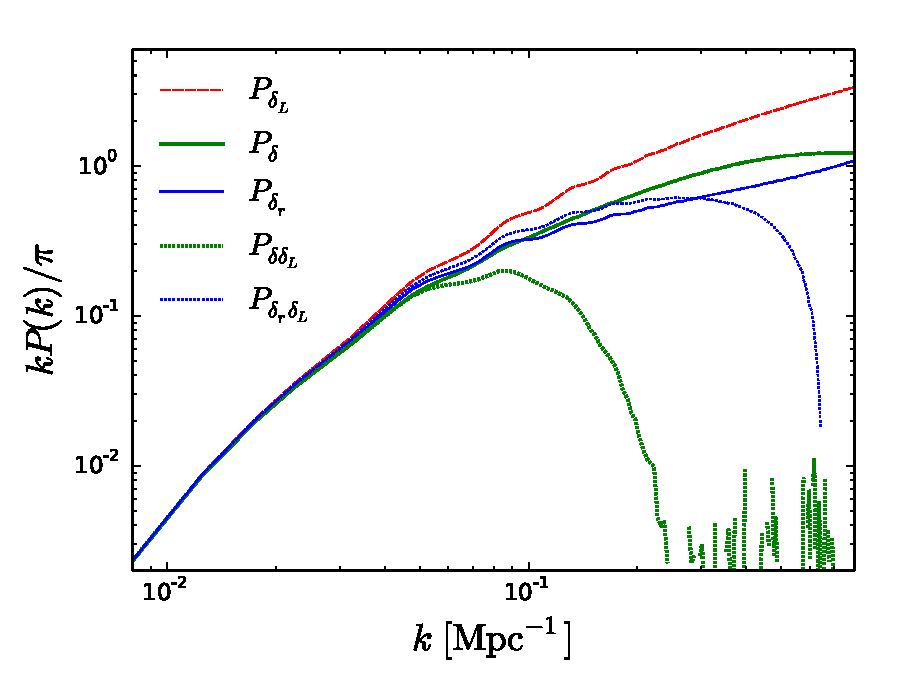
\includegraphics[width=0.48\textwidth]{f3x.eps}
\end{center}
\vspace{-0.7cm}
\caption{The power spectra of the linear (dashed line), nonlinear (thick solid
line), and reconstructed (thin solid line) fields. 
We also plot the nonlinear-linear (thick dotted line) and 
reconstructed-linear (thin dotted line) cross-correlation power spectra.
The wiggles in the reconstructed power spectrum are also much 
more transparent than the nonlinear power spectrum.}
\label{fig:ps}
\end{figure}

\begin{figure}[tbp]
\begin{center}
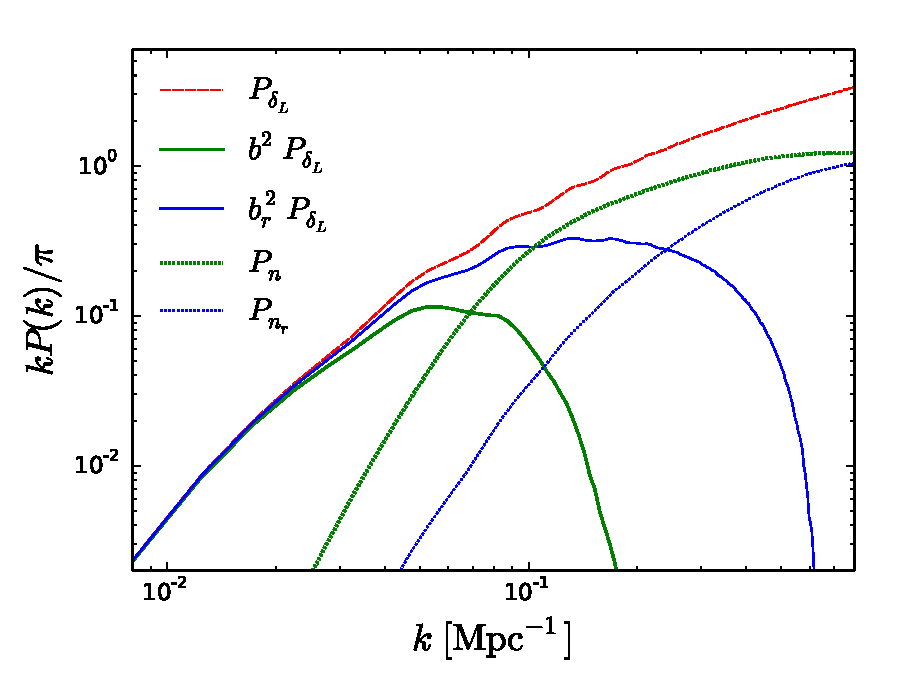
\includegraphics[width=0.48\textwidth]{f3xx.eps}
\end{center}
\vspace{-0.7cm}
\caption{The linear power spectrum (dashed line), the linear components in the
nonlinear (thick solid line) and reconstructed (thin solid line) fields,
the noise parts of the nonlinear (thick dotted line) and reconstructed (thin
dotted line) fields. The noise terms dominate over the signals at 
$k\gtrsim0.07\ \mr{Mpc}^{-1}$ for the nonlinear field and $k_q\gtrsim0.25\ \mr{Mpc}^{-1}$
for the reconstructed field.}
\label{fig:pn}
\end{figure}

To convenienty quantify the linear information $\delta_L$ in 
the nonlinear density field $\delta$, we decompose the nonlinear density field
$\delta$ as
\begin{eqnarray}
\delta({k})=b({k})\delta_L({k})+n({k}).
\end{eqnarray}
Here, $b\delta_L$ is completely correlated with the linear density field 
$\delta_L$ and $b=P_{\delta\delta_L}/P_{\delta_L}$.
Nonlinear evolution drives $b$ to drop from unity, reducing the linear signal.
$n$ is generated in the nonlinear evolution and thus uncorrelated with
the linear density field $\delta_L$, further reducing $b\delta_L$ with respect
to $\delta$. This part induces noises in the measurement of BAO. 
Hence we denote it as $n$. 
Such decomposition helps to write the nonlinear power spectrum as
\bea
P_\delta(k)=\mathcal{D}(k)P_{\delta_L}(k)+P_{n}(k),
\eea
where $\mathcal{D}=b^2$ describes the damping of the linear power specturm.
The reconstructed power spectrum $P_{\delta_r}$ can be describe in the 
same way.
Here, $b(k)$ is often referred as the ``propagator'' 
and $P_{n}$ is usually
called the mode-coupling term \cite{2006crocce,2008crocce,2008matsubara}.
In Fig. \ref{fig:pn}


\begin{figure}[tbp]
\begin{center}
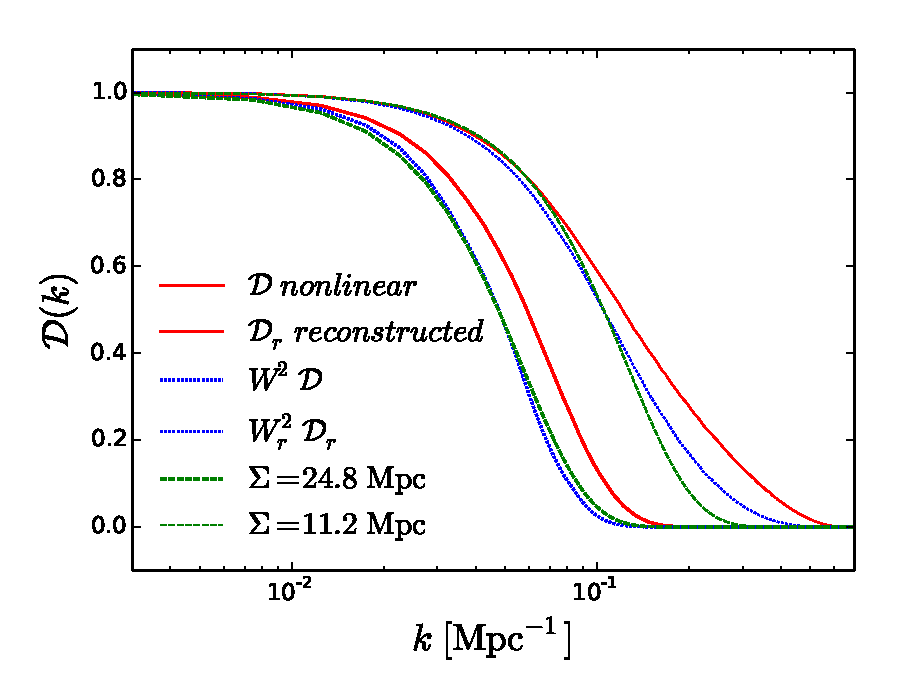
\includegraphics[width=0.48\textwidth]{f6x.eps}
\end{center}
\vspace{-0.7cm}
\caption{The damping factors for the nonlinear (thin solid line) and 
reconstructed (thick solid line) fields. The Gaussian BAO damping models with 
$\Sigma=20\ \mr{Mpc}$ (thick dotted line) and $\Sigma=10\ \mr{Mpc}$ (thin dotted
line).}
\label{fig:damp}
\end{figure}

Figure \ref{fig:damp} shows the damping functions for the raw and reconstructed 
fields. The nonlinear damping of the linear power spectrum is 
significantly reduced after reconstruction. We also overplot the best-fitting 
Gaussian BAO damping model,
\bea
\mathcal{D}(k)=\mr{e}^{-k^2\Sigma^2/2},
\eea
with $\Sigma=?\ \mr{Mpc}$ and $?\ \mr{Mpc}$ for the nonlinear and reconstructed 
fields. The new BAO reconstruction algorithm reduces the the nonlinear damping
scale $\Sigma$ by ?? per cent, i.e., a of ??. The damping factor is above 0.9
for $k\lesssim?\ \mr{Mpc}^{-1}$ indicating (almost) perfect reconstruction. 
\tcb{how to best quantify the reduction of damping? }
However, the 100 per cent reconstruction, cancelling any nonlinear effects,
is still unachievable, as some information has been irreversibly lost. (more 
discissions)

\begin{figure}[tbp]
\begin{center}
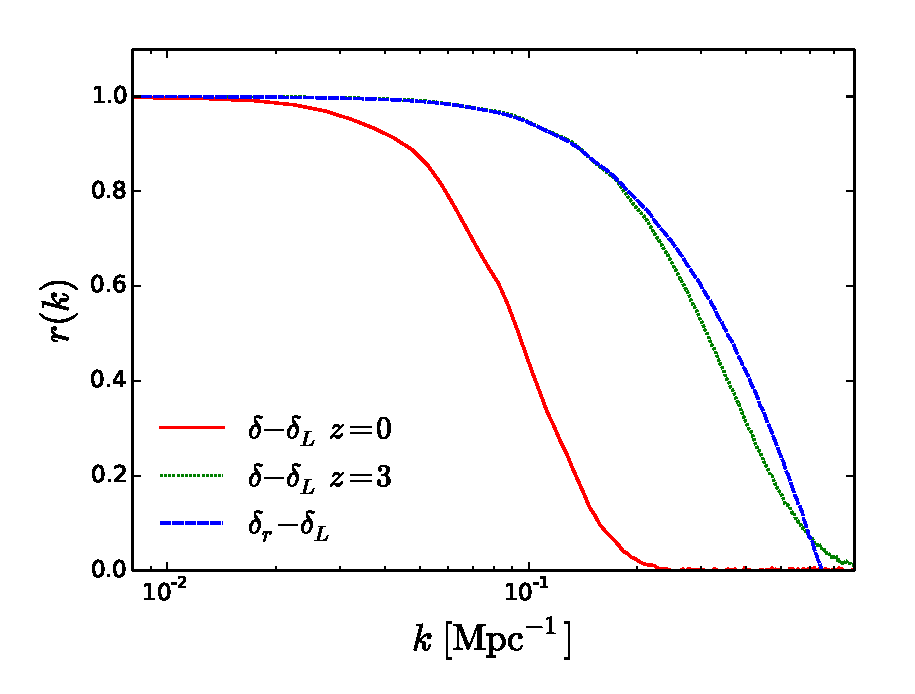
\includegraphics[width=0.48\textwidth]{f7x.eps}
\end{center}
\vspace{-0.7cm}
\caption{The $\delta-\delta_L$ correlation coefficients at $z=0$ (solid
line) and $z=3$ (dotted line), as well as the $\delta_r-\delta_L$ 
correlation coefficient (dashed line).}
\label{fig:xcc}
\end{figure}

Reconstruction also reduces the noise term $P_{\delta_N}$. To demonstrate this,
in Fig. \ref{fig:xcc} we plot the  cross-correltion coefficient 
\bea
r(k)=\frac{P_{\delta\delta_L}(k)}
{\sqrt{P_{\delta}(k)P_{\delta_L}(k)}}
=\frac{1}{\sqrt{1+\eta(k)}},
\eea
where $\eta=P_n/(\mathcal{D}P_{\delta_L})$ quantifies the relative amplitude
of $\delta_N$ with respect to $b\delta_L$. The correlation of $\delta_r$ with
$\delta_L$ is as good as that of $\delta$ at $z=3$.
\tcb{how to quantify this better?}

Distribution functions 
\begin{figure}[tbp]
\begin{center}
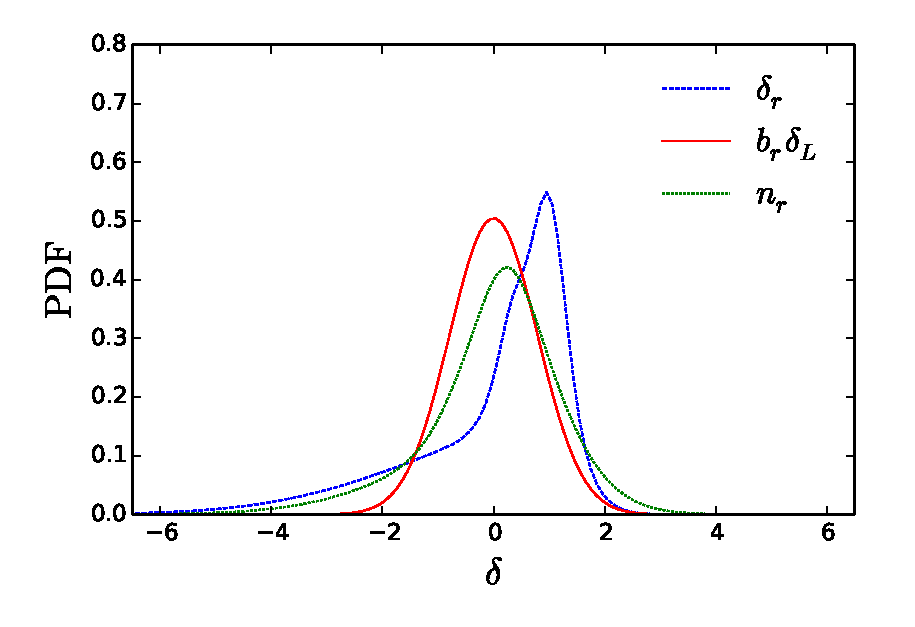
\includegraphics[width=0.48\textwidth]{f8x.eps}
\end{center}
\vspace{-0.7cm}
\caption{The distribution functions.}
\label{fig:pdf}
\end{figure}


%=======================================


\section{ Discussions}
The new method significantly
improves the expansion rate measurement from BAO. (more discussions?) 


This method can be generalized to the 3D case. 
We leave this
to future work.



Comparision with and Implications for the standard BAO reconstruction: exact 
Lagrangian displacement,
nonlinear displacement, which is easier to model.

If use the displacement solved in this paper for the standard BAO rec, we expect
the performance will become much better but still not as good as our results.
%=======================================

\section{Acknowledgement}
We acknowledge helpful discussions with Yu Yu and Tian-Xiang Mao.
We acknowledge the support of the Chinese MoST 863 program under Grant 
No. 2012AA121701, the CAS Science Strategic Priority Research Program 
XDB09000000, the NSFC under Grant No. 11373030, IAS at Tsinghua University, 
 and NSERC.
The Dunlap Institute is funded through an endowment established by the David Dunlap family and the University of Toronto.
Research at the Perimeter Institute is supported by the Government of Canada
through Industry Canada and by the Province of Ontario through the Ministry of
Research $\&$ Innovation.

\bibliographystyle{apsrev}
\bibliography{1d}

\end{document}
